
\documentclass[tikz,border=2mm]{standalone}
\usepackage[utf8]{inputenc}
\usepackage[T1]{fontenc}
\usepackage{amsmath}
\usepackage{amssymb}
\usetikzlibrary{arrows.meta,positioning,calc,shapes.geometric}
\usepackage{xcolor}

\definecolor{inkNavy}{HTML}{1B2733}
\definecolor{slate}{HTML}{3B4B5C}
\definecolor{paper}{HTML}{FBFAF7}
\definecolor{amber}{HTML}{C97A2B}
\definecolor{teal}{HTML}{2E7D74}
\definecolor{softred}{HTML}{A6402F}
\definecolor{lightgrey}{HTML}{E7E4DD}
\definecolor{midgrey}{HTML}{8B8A85}

\begin{document}
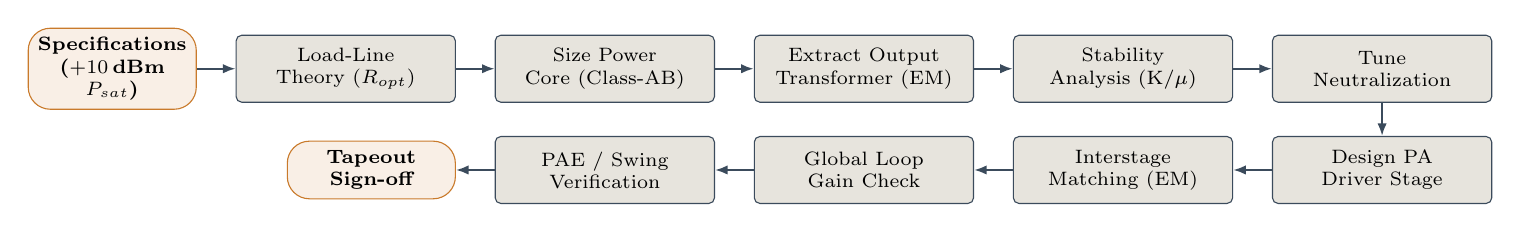
\begin{tikzpicture}[
  node distance=6pt and 14pt,
  box/.style={draw=slate, fill=lightgrey, rounded corners=2pt, text width=2.55cm, align=center, minimum height=0.85cm, font=\scriptsize},
  term/.style={draw=amber, fill=amber!12, rounded corners=8pt, text width=1.9cm, align=center, minimum height=0.7cm, font=\scriptsize\bfseries},
  arr/.style={-{Latex[length=1.6mm]}, slate, thick}
]
\node[term] (spec) {Specifications\\($+10$\,dBm $P_{sat}$)};
\node[box, right=of spec] (load) {Load-Line\\Theory ($R_{opt}$)};
\node[box, right=of load] (core) {Size Power\\Core (Class-AB)};
\node[box, right=of core] (xformer) {Extract Output\\Transformer (EM)};
\node[box, right=of xformer] (stab) {Stability\\Analysis (K/$\mu$)};
\node[box, right=of stab] (neut) {Tune\\Neutralization};

\node[box, below=12pt of neut] (driver) {Design PA\\Driver Stage};
\node[box, left=of driver] (match) {Interstage\\Matching (EM)};
\node[box, left=of match] (loop) {Global Loop\\Gain Check};
\node[box, left=of loop] (pvt) {PAE / Swing\\Verification};
\node[term, left=of pvt] (fin) {Tapeout\\Sign-off};

\draw[arr] (spec)--(load); \draw[arr] (load)--(core); \draw[arr] (core)--(xformer);
\draw[arr] (xformer)--(stab); \draw[arr] (stab)--(neut); \draw[arr] (neut)--(driver);
\draw[arr] (driver)--(match); \draw[arr] (match)--(loop); \draw[arr] (loop)--(pvt);
\draw[arr] (pvt)--(fin);
\end{tikzpicture}
\end{document}